\documentclass[a4paper,10pt]{beamer}
\usepackage{latexsym}
\usepackage[brazilian]{babel}
\usepackage{lmodern}
\usepackage[utf8]{inputenc}
\usepackage[T1]{fontenc}
\usepackage{longtable}
\usepackage{graphicx}

\usepackage{hyperref}
\usepackage{amsmath}  % for equation environment
% \usepackage{enumitem} % nolistsep to reduce list spacing
\usepackage{default}

\usepackage{listings}
\usepackage{color}

\lstset{ 
  basicstyle=\tiny\ttfamily,        % the size of the fonts for the code
  deletekeywords={path, data}, 
  frame=lines,
  showspaces = false,               % show spaces everywhere adding particular 
  showstringspaces = false,         % show spaces in string
  breaklines
%  title=\lstname                   % show the filename of files included with 
}

\begin{document}

\lstset{language=R}          % Set your language 

\begin{frame}
  \maketitle{Usando {\em R} para entender a COVID-19}
  
\end{frame}

\begin{frame}{Proposta da palestra}
  \begin{itemize}
      \item Visão geral da apresentação: foco em R, pandemia como motivação;
      \item Perfil do apresentador;
      \item Perfil esperado do público.
  \end{itemize}

\end{frame}

\begin{frame}{O que é o R ?}
  \begin{itemize}
      \item Biblioteca completa de estatística -- com acesso à 
	  Internet: Twitter;
      \item Software livre casa bem com academia;
      \item Ambiente expansível com bibliotecas de alto desempenho em C/C++;
      \item Linguagem interpretada de alto nível, especializada em estatística;
      \item Mundo à parte da estatística.
  \end{itemize}

\end{frame}

\begin{frame}{Características de uma pandemia}
  \begin{itemize}
      \item Processo exponencial;
      \item 1 pessoa contagia 10;
      \item 10 pessoas contagiam outras 10 cada uma;
      \item No passo $0$, $10^0 = 1 $ pessoa;
      \item No passo $1$, $10^1 = 10$ pessoas;
      \item No passo $2$, $10^2 = 100$ pessoas etc.
  \end{itemize}

\end{frame}

\begin{frame}[fragile]{Obtendo dados através do R}

  \lstinputlisting[title=\lstname]{scripts/get-full_data.R}
  \begin{itemize}
      \item uso de {\em snippets} para reduzir erros de digitação;
      \item endereçamento dos dados através de URL;
      \item normalmente (mesmo em Python) os dados seriam baixados em arquivo,
	  depois processados.
  \end{itemize}

\end{frame}

\begin{frame}{Filtragem dos dados da pandemia}
  \lstinputlisting[title=\lstname]{scripts/gen-work.R}
  
  \begin{itemize}
      \item Mas os dados do pacote de dados {\tt brazil} ainda não estão como 
	  necessário;
      \item O registro da pandemia no mundo começou no último dia de 2019;
      \item Mas no Brasil, ele começou apenas em fevereiro, início do 
	  primeiro caso.	  
      \item Filtra-se então o pacote {\tt brazil} para se ter o pacote de 
	  trabalho {\tt work};
      \item Usa-se a variável {\tt total\_cases} porque {\tt new\_cases} foi 
	  nula em alguns dias do início da pandemia.
  \end{itemize}

\end{frame}

\begin{frame}{Apresentação dos dados da pandemia ({\tt show\_work.R}) }
  \lstinputlisting[title=\lstname]{scripts/show-work.R}
  
  \begin{itemize}
      \item A função {\tt View(work)} apresenta os dados em uma 
	  planilha;
      \item A função  {\tt ncol(work)} informa quantas colunas há nesses
	  dados;
      \item A função  {\tt nrow(work)} informa quantas linhas há nesses
	  dados;
      \item A função  {\tt str(work)} informa a estrutura desses 
	  dados, além de permitir uma ``xereteda'' neles;
  \end{itemize}

\end{frame}

\begin{frame}{ Escolha de dados: {\tt new\_cases} e {\tt total\_cases} }
  \begin{itemize}
      \item Usaremos os casos de infecção, não de falecimentos, ou {\em deaths};
      \item As duas variáveis são relacionadas, mas os casos são em 
	  maior quantidade e, portanto, menos sujeitos a erros de medida.
      \item Contudo, resta decidir se devemos usar a ocorrência diária de 
	  novos casos ({\tt new\_cases}) ou seu valor acumulado 
	  {\tt total\_cases}.	
      \item Uma forma simples de avaliar variáveis é através de sua 
	  apresentação em gráfico -- sua ``plotagem'', ou {\em plot}.
  \end{itemize}

\end{frame}

\begin{frame}{ Criação de variável de apoio {\tt day}}
  \lstinputlisting[title=\lstname]{scripts/creat-day.R}
  
  \begin{itemize}
      \item Infelizmente, como vimos nas apresentações dos dados, as variáveis
	  de fator são preservadas nos subpacotes de dados;
	  
      \item Assim, a variável {\tt date} será sempre iniciada a partir de 
	  {\tt 2019-12-31}, não do início da pandemia.
	  
      \item Por isso criamos a variável {\tt day} que terá valor $1$ no 
	  primeiro dia da pandemia, e terá tantos elementos quanto os dias 
	  em que a pandemia foi registrada.
	  
      \item No {\em script} {\tt length(work\$total\_cases)} 
	  define o comprimento total (ou número de linhas) da variável 
	  {\tt total\_cases} do pacote de dados {\tt work} que estamos 
	  trabalhando;
      \item o cifrão {\tt \$} informa a subordinação entre {\tt work} e 
	  {\tt total\_cases}; ou seja: {\tt total\_cases} {\em pertence} 
	  ao pacote {\tt work}.
  \end{itemize}

\end{frame}

\begin{frame}{Plotagem de {\tt day} versus {\tt new\_cases}}
  \lstinputlisting[title=\lstname]{scripts/plot-new_cases.R}
  
  \begin{itemize}
      \item O programa é fácil de ser entendido ele desenha ({\em to plot})
	  duas variáveis: uma na abscissa (ou $x$) e outra na ordenada 
	  (ou $y$) -- respectivamente {\tt day} e 
	  {\tt work\$new\_cases}.
      \item Mas o desenho resultante é difícil de ser entendido: a partir 
	  dos primeiros 70 dias não há mais um padrão claro.
  \end{itemize}

\end{frame}

\begin{frame}{ Plotagem de {\tt day} versus {\tt new\_cases} ({\em cont}) }
   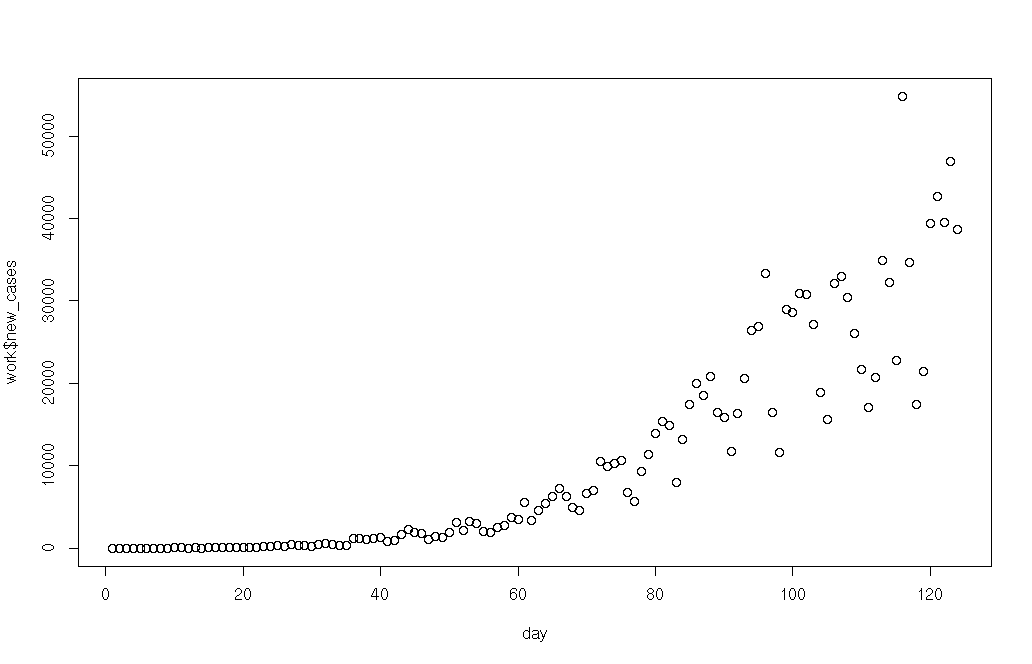
\includegraphics[scale=0.375]{plot-dayXnew_cases.png}

\end{frame}

\begin{frame}{ Plotagem de {\tt day} versus  {\tt total\_cases}}
  \lstinputlisting[title=\lstname]{scripts/plot-total_cases.R}
  
  \begin{itemize}
      \item A compreensão do programa é a mesma do caso anterior; naturalmente
	  substituindo {\tt new\_cases} por {\tt total\_cases}.
	  
      \item Mas é muito mais fácil ver um padrão na variável {\tt total\_cases}
	  do que na variável {\tt new\_cases}.
	  
      \item Por isso é com ela que seguiremos os estudos.
  \end{itemize}

\end{frame}

\begin{frame}{ Plotagem de {\tt day} versus {\tt total\_cases} ({\em cont}) }
  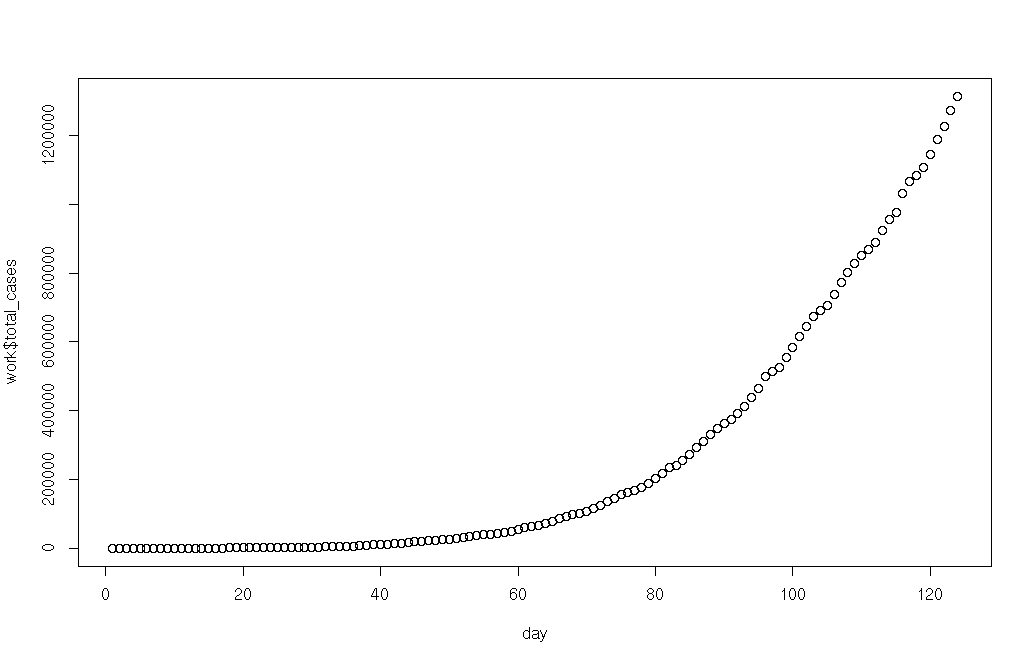
\includegraphics[scale=0.375]{plot-dayXtotal_cases.png}

\end{frame}

% \begin{frame}{ Regressão linear de {\tt day} versus  {\tt total\_cases}}
%   \lstinputlisting[title=\lstname]{scripts/plot-lin.R}
%   
%   \begin{itemize}
%       \item A regressão linear permite escolher a melhor reta da variável 
% 	  {\bf independente} {\tt day} para expressar a variável 
% 	  {\bf dependente} {\tt total\_cases};
%       \item Isto é feito em $R$ agregando-se ambas em uma {\em data frame};
%       \item Ajusta-se então um modelo linear, entre elas;
%       \item A seguir, apaga-se a tela;
%       \item Plota-se {\tt day} e {\tt total\_cases};
%       \item E a seguir a reta aproximada.
%   \end{itemize}
% 
% \end{frame}

% \begin{frame}{ Regressão linear de {\tt day} versus  {\tt total\_cases}
%     ({\em cont.}) }
%   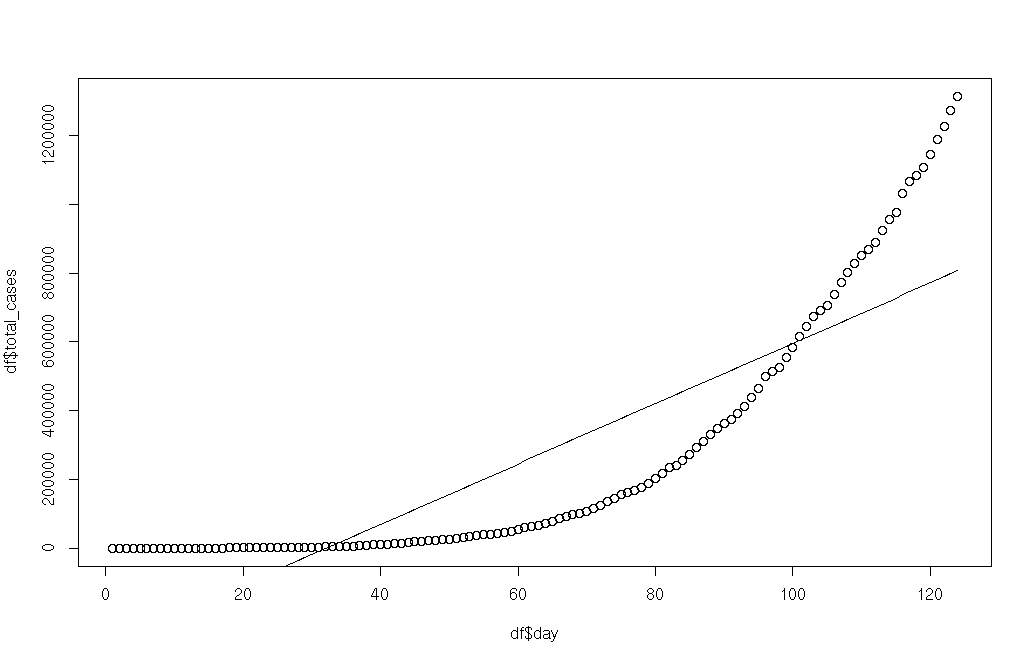
\includegraphics[scale=0.375]{plot-lin.png}
%   
% \end{frame}

\begin{frame}{O que é uma função exponencial}
  \begin{itemize}
      \item A função exponencial clássica é $y = e^x$, onde $e$ é a chamada
	  {\em constante de Euler}.
      \item Ela é muito importante para a matemática, mas neste caso estamos
	  interessados em sua propriedade de crescer muito rapidamente.
      \item Essa equação simples será reescrita como 
	  $T = e^{\alpha d + \beta}$.
      \item Seguindo o hábito dos matemáticos, de usar uma única letra para 
	  variáveis, $T$ significa {\tt total\_cases} e $d$ signfica
	  {\tt day}.
      \item $\alpha$ e $\beta$ são constantes que dão mais flexibilidade 
	  ao ajuste da função.
  \end{itemize}

\end{frame}

\begin{frame}{Uso de logaritmo para facilitar a regressão linear}
  \begin{itemize}
      \item Infelizmente, a técnica de regressão linear trabalha apenas com
	  retas, planos e similares.
      \item Para fazer surgir uma reta neste caso, aplica-se a função 
	  logaritmo nos dois lados da igualdade:
	  \begin{equation*}
	      log(T) = log(e^{\alpha d + \beta}) = \alpha d + \beta.
	  \end{equation*}

      \item a transformação de $log(e^{\alpha d + \beta})$ em $\alpha d + \beta$
	  é possível porque $log(x)$ e $e^x$ são funções inversas.
      \item Sua {\em composição} (aplicação sucessiva) é a 
	  {\em função identidade}.
      \item Ou seja: $log(e^x) = x$. Além disso, $e^{log(x)} = x$
  \end{itemize}

\end{frame}

\begin{frame}{ Regressão de {\tt day} versus $log(total\_cases)$}
  \lstinputlisting[title=\lstname]{scripts/plot-exp.R}
  
  \begin{itemize}
      \item Primeiro criamos a variável {\tt total\_cases\_log} transformando 
	  os valores de {\tt total\_cases} através da função $log()$;
      \item Depois criamos o {\em data frame} {\tt df\_exp} para a regressão.
      \item A seguir, plotamos as variáveis usadas e a reta aproximada.
  \end{itemize}

\end{frame}

\begin{frame}{ Regressão de {\tt day} versus $log(total\_cases)$
    ({\em cont.})}
  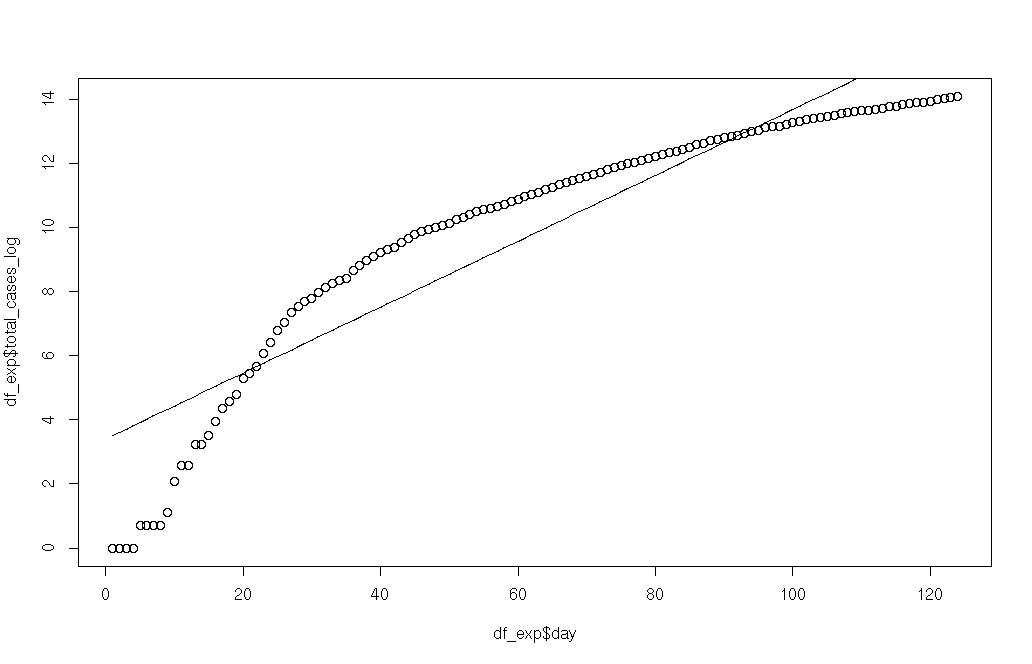
\includegraphics[scale=0.375]{plot-exp.png}
\end{frame}

% \begin{frame}{ Plotagem sem transformação logarítmica }
%   \lstinputlisting[title=\lstname]{scripts/plot-unexp.R}
%   
%   \begin{itemize}
%       \item Para avaliar a aproximação nos dados reais, converteremos os 
% 	  dados da regressão em dados reais, desfazendo a transformação
% 	  logarítica.
%       \item Como a função inversa de $log(x)$ é $e^x$, que se escreve
% 	  {\tt exp(x)} em $R$, isto é feito na primeira linha do 
% 	  {\em snippet}.
%   \end{itemize}
% 
% \end{frame}
% 
% \begin{frame}{ Plotagem sem transformação logarítmica ({\em cont.}) }
%   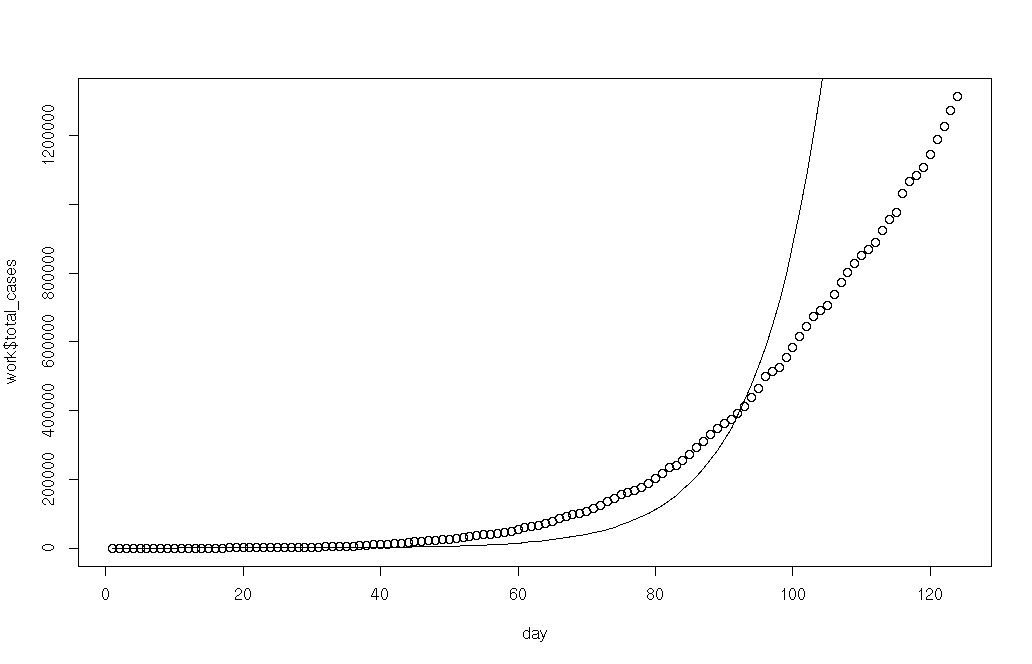
\includegraphics[scale=0.375]{plot-unexp.png}
% 
% \end{frame}

\begin{frame}{ Melhor aproximação $T = e^{\gamma d^2 + \delta d + \epsilon}$}
  \begin{itemize}
      \item Para melhorar o ajuste de uma função de {\tt day} à variável
	  dependente {\tt total\_cases}, incluiremos um termo quadrático.
      \item Ou seja: tentaremos expressar {\tt total\_cases} através de 
	  uma parábola de {\tt day}, em vez de simples reta.
      \item Uma parábola tem a vantagem de que seu crescimento é variável e 
	  podemos ajustá-la a trechos dos dados.
  \end{itemize}

\end{frame}

\begin{frame}{ Adição de {\tt $day^2$} à função exponencial}
  \lstinputlisting[title=\lstname]{scripts/plot-exp2.R}
  
  \begin{itemize}
      \item Primeiro se cria a variável {\tt day\_sq} como o quadrado da 
	  variável {\tt day}, ou o produto de {\tt day} por ela mesma;
      \item A seguir, cria-se a {\em data frame} {\tt df\_exp2} para 
	  conter todas variáveis da nova regressão;
      \item O novo modelo de regressão linear agora inclui {\tt day\_sq}.
      \item A seguir, plota-se {\tt day}, {\tt total\_cases} e a 
	  função aproximada, como feito antes.
	  
  \end{itemize}

\end{frame}

\begin{frame}{ Adição de {\tt $day^2$} à função exponencial ({\em cont.}) }
  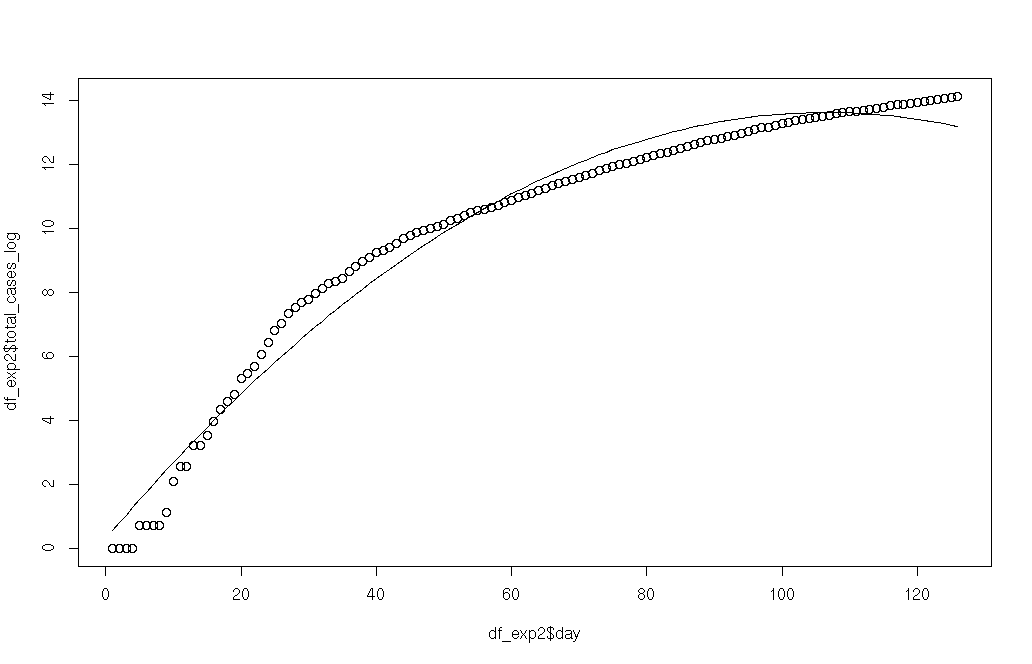
\includegraphics[scale=0.375]{plot-exp2.png}

\end{frame}

\begin{frame}{ Plotagem da exponencial quadrática sem transformação logarítmica}
  \lstinputlisting[title=\lstname]{scripts/plot-unlog2.R}
  
  \begin{itemize}
      \item Neste caso, como feito antes, usa-se a função exponencial para 
	  converter os dados aproximados em termos de {\tt total\_case}, não
	  mais de {\tt log(total\_case)}.
  \end{itemize}

\end{frame}


\begin{frame}{ Plotagem da exponencial quadrática sem transformação logarítmica
      ({\em cont.})}
  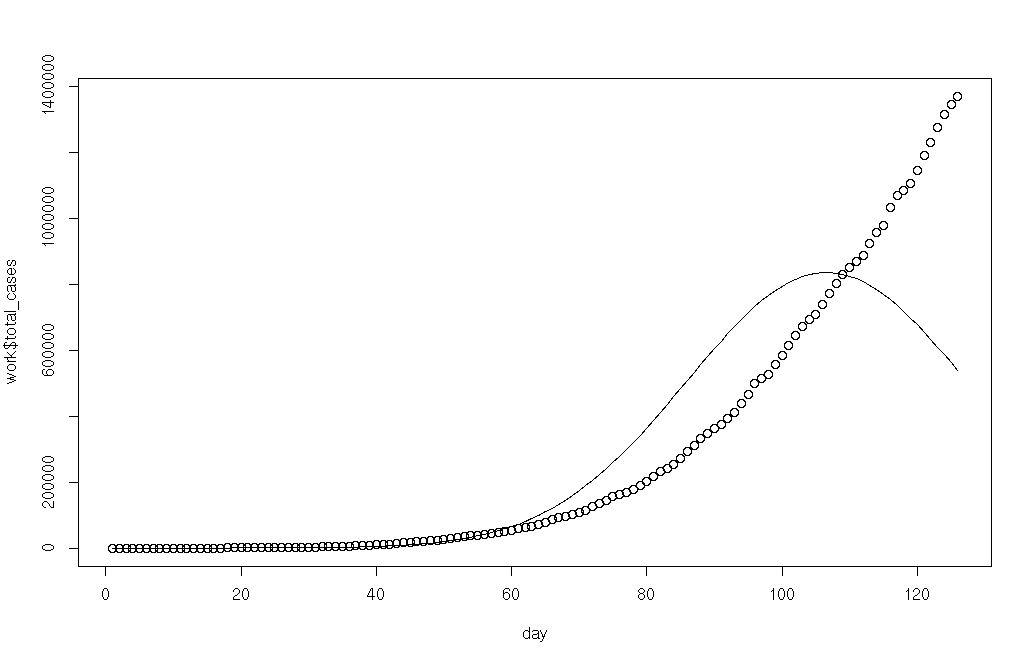
\includegraphics[scale=0.375]{plot-unexp2.png}

\end{frame}

\begin{frame}{ Estimativa do pico da pandemia }
  \lstinputlisting[title=\lstname]{scripts/calc-peak.R}
  
  \begin{itemize}
      \item Este {\em snippet} usa os coeficientes da parábola aproximada para 
	  estimar o pico da pandemia.
  \end{itemize}

\end{frame}

\end{document}
